%==============================================================================
%  LAB REPORT 5 — BMP280 Sensor Data Reading for Pressure, Temperature and Altitude
%  Compile with pdfLaTeX (works out of the box on Overleaf).
%
%  >>> PASTE YOUR GOOGLE DRIVE LINKS IN THE MACROS MARKED "EDIT ME" BELOW <<<
%==============================================================================
\documentclass[10pt,a4paper]{article}

%---------------------------------------- page geometry
\usepackage[a4paper,top=2.2cm,bottom=2.0cm,left=2.1cm,right=2.1cm,
            headsep=13pt,footskip=22pt]{geometry}

%---------------------------------------- encoding & fonts
\usepackage[T1]{fontenc}
\usepackage[utf8]{inputenc}
\usepackage{newtxtext,newtxmath}     % Times-like professional text + math
\usepackage[scaled=0.86]{beramono}   % clean monospace for code
\usepackage{microtype}

%---------------------------------------- graphics, colour, boxes
\usepackage{graphicx}
\usepackage[dvipsnames,table]{xcolor}
\usepackage{tikz}
\usepackage{circuitikz}
\usepackage{pgfplots}
\pgfplotsset{compat=1.18}
\usepgfplotslibrary{groupplots}
\usepackage[most]{tcolorbox}
\usepackage{booktabs}
\usepackage{array}
\usepackage{tabularx}
\usepackage{enumitem}
\usepackage{listings}
\usepackage{fancyhdr}
\usepackage{titlesec}
\usepackage{caption}
\usepackage{float}
\usepackage{needspace}
\usetikzlibrary{arrows.meta,positioning,calc,shadows.blur,decorations.pathreplacing}
\ctikzset{bipoles/length=0.62cm}   % compact component symbols

%---------------------------------------- hyperlinks (load late)
\usepackage[hidelinks]{hyperref}
\usepackage{url}
% print a URL stored in a macro, safely (handles _ ~ % etc.)
\newcommand{\showurl}[1]{\expandafter\url\expandafter{#1}}

%==============================================================================
%  Student details
%==============================================================================
\newcommand{\studentname}{Chavan Atharva Sunil}
\newcommand{\rollnumber}{240003021}
\newcommand{\coursecode}{AA303 --- IoT for Space Applications}
\newcommand{\expdate}{3 September 2026 (ESP32) and 10 September 2026 (Raspberry Pi)}   % <-- CHECK THE PI DATE

%  Google Drive folder holding the demonstration videos and the source code
\urldef{\drivefolder}\url{https://drive.google.com/drive/folders/11TP-NX_EF_IpxHlAUYmG8YWPQfst2ae2?usp=sharing}

%==============================================================================
%  Colour palette
%==============================================================================
\definecolor{ink}{HTML}{1B2733}      % body text / headings
\definecolor{accent}{HTML}{0B5FA5}   % primary blue
\definecolor{accentlt}{HTML}{E8F1FA} % pale blue fill
\definecolor{amber}{HTML}{C8791A}    % LED amber
\definecolor{amberlt}{HTML}{FDF3E3}
\definecolor{rule}{HTML}{C9D4DE}
\definecolor{soft}{HTML}{F5F7F9}
\definecolor{codebg}{HTML}{F7F9FB}
\definecolor{cmnt}{HTML}{6C8090}
\definecolor{kw}{HTML}{0B5FA5}
\definecolor{str}{HTML}{1C7C54}
\definecolor{num}{HTML}{9B2D5E}

\color{ink}

%==============================================================================
%  Headings
%==============================================================================
\titleformat{\section}
  {\normalfont\large\bfseries\color{accent}}
  {\raisebox{0pt}{\colorbox{accent}{\color{white}\bfseries\;\thesection\;}}}
  {0.7em}{}[\vspace{2pt}{\color{rule}\titlerule[0.8pt]}]
\titlespacing*{\section}{0pt}{14pt}{8pt}

\titleformat{\subsection}
  {\normalfont\normalsize\bfseries\color{ink}}{\thesubsection}{0.6em}{}
\titlespacing*{\subsection}{0pt}{11pt}{4pt}

\titleformat{\subsubsection}
  {\normalfont\small\bfseries\color{accent}}{}{0em}{}
\titlespacing*{\subsubsection}{0pt}{9pt}{2pt}

%==============================================================================
%  Header / footer
%==============================================================================
\pagestyle{fancy}
\fancyhf{}
\renewcommand{\headrulewidth}{0.4pt}
\renewcommand{\footrulewidth}{0pt}
\fancyhead[L]{\footnotesize\color{cmnt}\textsc{Lab Report 5} \,\textbar\, BMP280 Pressure, Temperature and Altitude}
\fancyhead[R]{\footnotesize\color{cmnt}\studentname\ \,\textbar\, \rollnumber}
\fancyfoot[C]{\footnotesize\color{cmnt}\thepage}

%==============================================================================
%  Captions & lists
%==============================================================================
\captionsetup{font=small,labelfont={bf,color=accent},skip=6pt}
\setlist[itemize]{leftmargin=1.35em,itemsep=2pt,topsep=3pt}
\setlist[enumerate]{leftmargin=1.6em,itemsep=2.5pt,topsep=3pt}
\renewcommand{\arraystretch}{1.18}

%==============================================================================
%  Custom boxes
%==============================================================================
\newtcolorbox{keybox}[1][]{
  enhanced, breakable, colback=accentlt, colframe=accent,
  boxrule=0pt, leftrule=3pt, arc=2pt, left=10pt, right=10pt, top=8pt, bottom=8pt,
  fontupper=\normalsize, #1}

\newtcolorbox{notebox}[1][]{
  enhanced, breakable, colback=amberlt, colframe=amber,
  boxrule=0pt, leftrule=3pt, arc=2pt, left=10pt, right=10pt, top=7pt, bottom=7pt,
  fontupper=\small, #1}

\newtcolorbox{titledbox}[2][]{
  enhanced, breakable, colback=white, colframe=rule, boxrule=0.6pt, arc=3pt,
  left=10pt, right=10pt, top=8pt, bottom=8pt,
  title={\bfseries\small #2}, coltitle=white, colbacktitle=accent,
  attach boxed title to top left={xshift=8pt,yshift=-8pt},
  boxed title style={boxrule=0pt,arc=2pt,left=6pt,right=6pt,top=2pt,bottom=2pt},
  #1}

%==============================================================================
%  Code listing style
%==============================================================================
\lstdefinestyle{prostyle}{
  backgroundcolor=\color{codebg},
  basicstyle=\ttfamily\scriptsize\color{ink},
  keywordstyle=\color{kw}\bfseries,
  commentstyle=\color{cmnt}\itshape,
  stringstyle=\color{str},
  numberstyle=\ttfamily\tiny\color{cmnt},
  numbers=left, numbersep=9pt, xleftmargin=17pt, xrightmargin=2pt,
  frame=single, framesep=6pt, rulecolor=\color{rule},
  breaklines=true, showstringspaces=false, tabsize=2,
  columns=fullflexible, keepspaces=true,
  aboveskip=8pt, belowskip=6pt,
  emphstyle=\color{num}\bfseries,
  literate={°}{{$^{\circ}$}}1
}
\lstset{style=prostyle}

%==============================================================================
%  Schematic: I2C connection from a board's header to the BMP280 breakout
%  \iicschematic{board}{vcc pin}{sda pin}{scl pin}{gnd pin}
%==============================================================================
\newcommand{\iicschematic}[5]{%
\begin{circuitikz}[scale=0.71, transform shape, every node/.style={font=\footnotesize}]
  % ---- controller
  \draw[fill=accentlt, draw=accent, line width=0.9pt, rounded corners=4pt]
        (-3.5,-0.45) rectangle (-0.6,4.15);
  \node[text=accent, font=\small\bfseries] at (-2.05,3.65) {#1};
  \node[text=cmnt,   font=\scriptsize]     at (-2.05,3.25) {I$^2$C master};
  \foreach \y/\pin/\name in {2.55/#2/3.3\,V, 1.75/#3/SDA, 0.95/#4/SCL, 0.15/#5/GND}{
     \draw[fill=white, draw=accent, line width=0.6pt] (-0.92,\y-0.14) rectangle (-0.6,\y+0.14);
     \node[anchor=east, font=\scriptsize\bfseries, text=accent, align=right] at (-1.02,\y) {\pin\\[-2pt]{\tiny\color{cmnt}\name}};}
  % ---- wires
  \draw[line width=1.1pt, red!70!black] (-0.6,2.55) -- (3.0,2.55);
  \draw[line width=1.1pt, violet]       (-0.6,1.75) -- (3.0,1.75);
  \draw[line width=1.1pt, gray]         (-0.6,0.95) -- (3.0,0.95);
  \draw[line width=1.1pt, black]        (-0.6,0.15) -- (3.0,0.15);
  \node[font=\tiny, text=red!70!black, anchor=south] at (1.2,2.6)  {VCC};
  \node[font=\tiny, text=violet,       anchor=south] at (1.2,1.8)  {SDA --- data};
  \node[font=\tiny, text=gray!60!black,anchor=south] at (1.2,1.0)  {SCL --- clock};
  \node[font=\tiny, text=cmnt,         anchor=south] at (1.2,0.2)  {GND};
  % ---- breakout module
  \draw[fill=soft, draw=rule, line width=0.8pt, rounded corners=4pt] (3.0,-0.45) rectangle (7.9,4.15);
  \node[text=ink, font=\small\bfseries] at (5.45,3.7) {BMP280 breakout};
  \node[text=cmnt, font=\scriptsize] at (5.45,3.33) {six-pin module, I$^2$C mode};
  \foreach \y/\lab in {2.55/VCC, 1.75/SDA, 0.95/SCL, 0.15/GND}{
     \draw[fill=white, draw=ink, line width=0.6pt] (3.0,\y-0.14) rectangle (3.32,\y+0.14);
     \node[anchor=west, font=\tiny\bfseries] at (3.34,\y) {\lab};}
  % on-board pull-ups from VCC to SDA and SCL
  \draw[line width=0.7pt] (3.32,2.55) -- (4.3,2.55);
  \draw[line width=0.7pt] (4.3,2.55) -- (4.3,2.45) to[R, l_=$10\,\mathrm{k}\Omega$] (4.3,1.75);
  \draw[line width=0.7pt] (4.3,2.55) -- (5.0,2.55) -- (5.0,2.45) to[R] (5.0,0.95);
  \draw[line width=0.7pt] (3.32,1.75) -- (4.3,1.75) -- (6.2,1.75);
  \draw[line width=0.7pt] (3.32,0.95) -- (5.0,0.95) -- (6.2,0.95);
  \draw[line width=0.7pt] (5.0,2.55) -- (6.2,2.55);
  \draw[line width=0.7pt] (3.32,0.15) -- (6.2,0.15);
  \fill (4.3,2.55) circle (1.2pt); \fill (5.0,2.55) circle (1.2pt);
  \fill (4.3,1.75) circle (1.2pt); \fill (5.0,0.95) circle (1.2pt);
  % sensor body
  \draw[fill=cyan!20, draw=cyan!60!black, line width=0.8pt] (6.2,-0.2) rectangle (7.7,2.95);
  \node[font=\scriptsize\bfseries, text=cyan!40!black, rotate=90] at (7.35,1.4) {BMP280};
  \node[font=\tiny, anchor=west] at (6.22,2.72) {VDD};
  \node[font=\tiny, anchor=west] at (6.22,1.92) {SDI};
  \node[font=\tiny, anchor=west] at (6.22,1.12) {SCK};
  \node[font=\tiny, anchor=west] at (6.22,0.32) {GND};
  \node[font=\tiny, text=cmnt, anchor=north] at (5.45,-0.5) {SDO tied to GND on the module $\Rightarrow$ address 0x76};
\end{circuitikz}}

%==============================================================================
\begin{document}

%------------------------------------------------------------------ TITLE BLOCK
\thispagestyle{empty}
\begin{tikzpicture}[remember picture, overlay]
  \fill[accent] (current page.north west) rectangle
        ($(current page.north east)+(0,-7.15cm)$);
  \fill[amber] ($(current page.north west)+(0,-7.15cm)$) rectangle
        ($(current page.north east)+(0,-7.3cm)$);
\end{tikzpicture}

\vspace*{0.35cm}
{\color{white}
 \noindent{\footnotesize\textsc{\coursecode}}\\[2pt]
 \noindent{\Large\bfseries Experiment 5 \,\textbar\, Lab Report}\\[8pt]
 \noindent{\huge\bfseries BMP280 Sensor Data Reading}\\[6pt]
 \noindent{\LARGE\bfseries for Pressure, Temperature and Altitude}\\[10pt]
 \noindent{\small Reading a barometric sensor over I$^2$C on a Raspberry Pi, and publishing it from an ESP32 as a live web dashboard}
}
\vspace{1.5cm}

\noindent
\begin{tabularx}{\textwidth}{@{}>{\bfseries\color{accent}}l X@{}}
\toprule
Submitted by  & \studentname \\
Roll Number   & \rollnumber \\
Date of Experiment & \expdate \\
Boards Used   & Raspberry Pi 4 (I$^2$C bus 1, GPIO2/GPIO3) and ESP32 DevKit (I$^2$C on GPIO21/GPIO22) \\
\bottomrule
\end{tabularx}

\vspace{10pt}

%------------------------------------------------------------------ 1. AIM
\section{Aim}

\begin{keybox}
To read \textbf{atmospheric pressure} and \textbf{temperature} from a \textbf{BMP280}
barometric sensor over the \textbf{I$^2$C} bus, and to derive the \textbf{altitude}
from the pressure. The sensor is read first from a \textbf{Raspberry Pi}, printing a
new set of values to the terminal every second, and then from an \textbf{ESP32}, which
hosts its own Wi-Fi access point and serves a web page that shows the three quantities
live in a browser.
\end{keybox}

\subsection*{Objectives}
\begin{itemize}
  \item To connect a BMP280 breakout module to a Raspberry Pi and to an ESP32 over the
        two-wire I$^2$C bus and identify it at its address \texttt{0x76}.
  \item To read the compensated pressure and temperature from the sensor with a
        driver library on each board, and to convert the pressure into an altitude
        with the barometric formula.
  \item To present the readings in two ways: as a continuously updating terminal
        printout on the Pi, and as a web dashboard served by the ESP32 to any device
        that joins its Wi-Fi network.
  \item To compare the pressure and pressure-altitude recorded on two different days
        at the same place, and to understand what the ``altitude'' of a barometer
        actually measures.
\end{itemize}

\subsection*{Brief Theory}
The BMP280 is a digital barometric pressure sensor from Bosch. A piezo-resistive
sensing element and a temperature sensor feed a 24-bit ADC; the chip's own factory
calibration constants, stored in its non-volatile memory, are read out by the driver
and used to \emph{compensate} the raw values into a temperature in $^{\circ}$C and a
pressure in Pa. It measures $300$--$1100\,\mathrm{hPa}$ with an absolute accuracy of
about $\pm1\,\mathrm{hPa}$ and a \emph{relative} accuracy of $\pm0.12\,\mathrm{hPa}$,
which corresponds to a height change of about one metre --- fine enough to notice the
sensor being raised from a desk to head height.

Pressure falls with height in a known way, so a barometer can be turned into an
altimeter. With the standard-atmosphere sea-level pressure $p_0 = 1013.25\,\mathrm{hPa}$
the height is
\[
  h = 44330\,\Bigl[\,1 - \Bigl(\frac{p}{p_0}\Bigr)^{1/5.255}\Bigr]\ \mathrm{m},
\]
which both driver libraries use. The result is a \emph{pressure altitude}: it is only
the true altitude if the sea-level pressure on the day really is $p_0$. Weather moves
$p_0$ by tens of hectopascals, and every hectopascal shifts the computed height by
roughly $8.5\,\mathrm{m}$ near sea level --- a point that the two runs in this report
illustrate directly.

\subsubsection{The I$^2$C bus}
Unlike the DHT11 of Experiment~4, which needed a bit-banged one-wire protocol with
microsecond timing, the BMP280 speaks the standard \textbf{I$^2$C} protocol, which both
boards support in hardware. Two lines are shared by every device on the bus: SDA (data)
and SCL (clock). Both are open-drain and held HIGH by pull-up resistors --- here the
ones on the breakout module --- and any device can only pull them LOW. The master
(the Pi or the ESP32) generates the clock and starts each transaction by sending the
7-bit address of the device it wants to talk to; the BMP280 answers on \texttt{0x76}
when its SDO pin is tied to ground (\texttt{0x77} if tied to VCC). Reading the sensor is
then a matter of writing a register address and reading back the bytes, which the
library handles.

\begin{notebox}
\textbf{Same pins, opposite setting.} On the Raspberry Pi the I$^2$C bus uses GPIO2
(SDA) and GPIO3 (SCL) --- the same GPIO2 that Experiment~4 drove as a plain output.
For the DHT11 the I$^2$C interface had to be \emph{disabled} in \texttt{raspi-config}
to free the pin; for the BMP280 it must be \emph{enabled}, after which the sensor
appears in \texttt{i2cdetect -y 1} at address \texttt{0x76}. On the ESP32 the default
I$^2$C pins are GPIO21 (SDA) and GPIO22 (SCL).
\end{notebox}

%------------------------------------------------------------------ 2. MATERIALS
\Needspace{8\baselineskip}
\section{Materials Required}

\noindent
\begin{tabularx}{\textwidth}{@{}p{0.4cm} >{\raggedright\arraybackslash}p{5.6cm} c X@{}}
\toprule
\rowcolor{soft}
\multicolumn{1}{@{}l}{\textbf{\#}} & \textbf{Component} & \textbf{Qty.} & \textbf{Purpose in the setup} \\
\midrule
1 & Raspberry Pi 4 (in case, with SD card, OS installed) & 1 & Part A host; I$^2$C master, prints readings to the terminal \\
2 & ESP32 DevKit (30-pin)                                 & 1 & Part B host; I$^2$C master, Wi-Fi access point and web server \\
3 & BMP280 breakout module (six-pin: VCC, GND, SCL, SDA, CSB, SDO) & 1 & Measures pressure and temperature; shared between the two parts \\
4 & Female--female jumper wires                            & 4 & VCC, GND, SDA and SCL between header and module \\
5 & Micro-USB cable and laptop with Arduino IDE and Wi-Fi & 1 & Programming the ESP32 and viewing the dashboard \\
6 & USB-C power supply, monitor, keyboard and mouse        & 1 & Running and observing the Raspberry Pi \\
7 & Software: \texttt{adafruit-circuitpython-bmp280} (Pi); \texttt{Adafruit BMP280} library and ESP32 core (Arduino IDE) & --- & Sensor drivers on the two boards \\
\bottomrule
\end{tabularx}

%------------------------------------------------------------------ 3. METHODOLOGY
\section{Methodology}

The same breakout module was used on both boards, wired the same way each time: four
jumper wires for VCC ($3.3\,\mathrm{V}$), GND, SDA and SCL, with the module's CSB and
SDO pins left as the board sets them (I$^2$C mode, address \texttt{0x76}). No
breadboard or extra components were needed because the pull-up resistors are on the
module.

\subsection{Connections}

\vspace{2pt}
\noindent
\begin{tabularx}{\textwidth}{@{}l l l >{\raggedright\arraybackslash}X@{}}
\toprule
\rowcolor{soft}
\textbf{Module pin} & \textbf{Raspberry Pi 4 (Part A)} & \textbf{ESP32 (Part B)} & \textbf{Function} \\
\midrule
VCC & Pin 1 --- $3.3\,\mathrm{V}$ & 3V3            & Supply (the BMP280 is a $3.3\,\mathrm{V}$ part) \\
GND & Pin 6 --- GND               & GND            & Ground \\
SDA & Pin 3 --- GPIO2 (\texttt{board.SDA}) & GPIO21 (\texttt{Wire} default) & Serial data, bidirectional \\
SCL & Pin 5 --- GPIO3 (\texttt{board.SCL}) & GPIO22 (\texttt{Wire} default) & Serial clock from the master \\
CSB, SDO & not connected & not connected & Module defaults: I$^2$C mode, address \texttt{0x76} \\
\bottomrule
\end{tabularx}

\begin{figure}[htb]
\centering
\begin{minipage}[t]{0.49\textwidth}
\centering
\iicschematic{Raspberry Pi}{Pin 1}{Pin 3}{Pin 5}{Pin 6}
\end{minipage}\hfill
\begin{minipage}[t]{0.49\textwidth}
\centering
\iicschematic{ESP32}{3V3}{GPIO21}{GPIO22}{GND}
\end{minipage}
\caption{Circuit schematics for the two parts. The wiring is identical apart from the
pin names: four wires, with the bus pull-ups and the address-setting SDO connection
already on the breakout module.}
\label{fig:schematic}
\end{figure}

\subsection{Part A --- Raspberry Pi, readings on the terminal}

With I$^2$C enabled, the sensor was confirmed on the bus with \texttt{i2cdetect -y 1}
and the Adafruit CircuitPython driver was installed:

\begin{lstlisting}[language=bash, caption={Preparing the Raspberry Pi.}, label={lst:install}]
sudo raspi-config          # Interface Options -> I2C -> Enable
sudo apt install i2c-tools
i2cdetect -y 1             # the BMP280 shows up at 0x76
pip3 install adafruit-circuitpython-bmp280
\end{lstlisting}

\noindent The program (Listing~\ref{lst:pi}) opens the bus, creates the sensor object
at \texttt{0x76}, sets the sea-level reference to $1013.25\,\mathrm{hPa}$, and then loops
once a second reading the three properties \texttt{temperature}, \texttt{pressure} and
\texttt{altitude} and printing them.

\Needspace{18\baselineskip}
\begin{lstlisting}[language=Python, caption={Part A --- \texttt{pressure.py} on the Raspberry Pi: temperature, pressure and altitude every second.}, label={lst:pi}]
import time
import board
import busio
import adafruit_bmp280

# Initialize I2C
i2c = busio.I2C(board.SCL, board.SDA)

# BMP280 sensor
bmp280 = adafruit_bmp280.Adafruit_BMP280_I2C(
    i2c,
    address=0x76
)

# Reference pressure at your starting location
# Change this if you want better altitude accuracy
bmp280.sea_level_pressure = 1013.25

while True:
    temperature = bmp280.temperature
    pressure = bmp280.pressure
    altitude = bmp280.altitude

    print("------------------------------")
    print(f"Temperature : {temperature:.2f} °C")
    print(f"Pressure    : {pressure:.2f} hPa")
    print(f"Altitude    : {altitude:.2f} m")

    time.sleep(1)
\end{lstlisting}


\subsection{Part B --- ESP32, readings on a web dashboard}

On the ESP32 the sensor is read with the Adafruit BMP280 Arduino library, but instead
of printing to a serial monitor the board publishes the values over Wi-Fi. The sketch
(Listing~\ref{lst:esp}) starts the ESP32 as a Wi-Fi \textbf{access point} --- it creates
its own network, so no router is needed --- and runs a small web server on it. The
server answers two requests: \texttt{/} returns the dashboard page, and \texttt{/data}
returns the current readings as a short JSON object. A few lines of JavaScript in the
page fetch \texttt{/data} every second and write the numbers into three cards, so a
laptop or phone that joins the ESP32's network and opens \texttt{http://192.168.4.1}
sees the readings update live.

\begin{figure}[H]
\centering
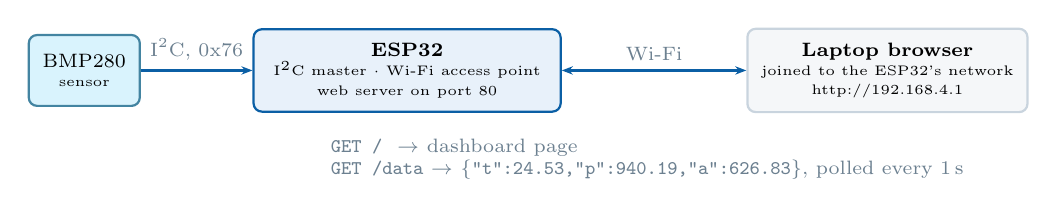
\begin{tikzpicture}[x=1cm, y=1cm, every node/.style={font=\scriptsize}]
  \tikzset{blk/.style={draw=accent, fill=accentlt, line width=0.8pt, rounded corners=3pt,
                       minimum height=0.9cm, align=center, inner sep=5pt}}
  \node[blk, fill=cyan!15, draw=cyan!60!black] (s) at (0,0) {BMP280\\[-1pt]{\tiny sensor}};
  \node[blk, minimum width=3.9cm] (e) at (4.1,0) {\textbf{ESP32}\\[-1pt]{\tiny I$^2$C master $\cdot$ Wi-Fi access point}\\[-1pt]{\tiny web server on port 80}};
  \node[blk, fill=soft, draw=rule, minimum width=3.2cm] (l) at (10.2,0) {\textbf{Laptop browser}\\[-1pt]{\tiny joined to the ESP32's network}\\[-1pt]{\tiny http://192.168.4.1}};
  \draw[-{Stealth[length=4pt]}, line width=0.8pt, accent] (s) -- node[above, text=cmnt]{I$^2$C, 0x76} (e);
  \draw[{Stealth[length=4pt]}-{Stealth[length=4pt]}, line width=0.8pt, accent] (e) -- node[above, text=cmnt]{Wi-Fi} (l);
  \node[anchor=north, text=cmnt, align=left] at (7.15,-0.75)
        {\texttt{GET /}\ \ $\to$ dashboard page\\ \texttt{GET /data} $\to$ \texttt{\{"t":24.53,"p":940.19,"a":626.83\}}, polled every 1\,s};
\end{tikzpicture}
\caption{Part B. The ESP32 reads the sensor over I$^2$C and serves the values over its
own Wi-Fi network; the page in the browser polls the JSON endpoint once a second.}
\label{fig:arch}
\end{figure}

\Needspace{18\baselineskip}
\begin{lstlisting}[language=C++, caption={Part B --- ESP32 sketch: BMP280 over I$^2$C, served as a live web dashboard from the board's own access point.}, label={lst:esp}]
#include <WiFi.h>
#include <WebServer.h>
#include <Wire.h>
#include <Adafruit_BMP280.h>

const char *AP_SSID = "ESP32-Sensor";     // the ESP32 creates this Wi-Fi network
const char *AP_PASS = "12345678";
const float SEA_LEVEL_HPA = 1013.25;      // reference for the altitude calculation

Adafruit_BMP280 bmp;                      // I2C, default pins SDA = 21, SCL = 22
WebServer server(80);

// The dashboard page. Its script asks the ESP32 for fresh values once per second.
const char PAGE[] PROGMEM = R"html(
<!DOCTYPE html><html><head><meta charset="utf-8">
<meta name="viewport" content="width=device-width,initial-scale=1">
<title>ESP32 Sensor</title>
<style>
 body{font-family:sans-serif;background:#1c2738;color:#ddd;text-align:center}
 h1{color:#4fc3f7} #st{color:#69e069}
 .card{background:#2b3a50;border-radius:10px;width:230px;margin:14px auto;padding:10px}
 .v{color:#69e069;font-size:30px;font-weight:bold} .u{font-size:12px;color:#aaa}
</style></head><body>
<h1>ESP32 Sensor Monitor</h1><div id="st">&#9679; ESP32 Connected</div>
<div class="card">Temperature<div class="v" id="t">--</div><div class="u">&deg;C</div></div>
<div class="card">Pressure<div class="v" id="p">--</div><div class="u">hPa</div></div>
<div class="card">Altitude<div class="v" id="a">--</div><div class="u">meters</div></div>
<script>
setInterval(async () => {
  try {
    const d = await (await fetch('/data')).json();
    t.textContent = d.t.toFixed(2);
    p.textContent = d.p.toFixed(2);
    a.textContent = d.a.toFixed(2);
    st.textContent = '\u25CF ESP32 Connected';    st.style.color = '#69e069';
  } catch (e) {
    st.textContent = '\u25CF ESP32 Disconnected'; st.style.color = '#ff7070';
  }
}, 1000);
</script></body></html>)html";

void handleRoot() { server.send_P(200, "text/html", PAGE); }

void handleData() {                       // the three readings as one JSON object
  float t = bmp.readTemperature();                 // degrees Celsius
  float p = bmp.readPressure() / 100.0F;           // Pa -> hPa
  float a = bmp.readAltitude(SEA_LEVEL_HPA);       // metres
  String json = "{\"t\":";  json += String(t, 2);
  json += ",\"p\":";        json += String(p, 2);
  json += ",\"a\":";        json += String(a, 2);  json += "}";
  server.send(200, "application/json", json);
}

void setup() {
  Serial.begin(115200);
  Wire.begin(21, 22);                              // SDA, SCL
  if (!bmp.begin(0x76)) {
    Serial.println("BMP280 not found - check the wiring and the address");
    while (true) delay(10);
  }
  WiFi.softAP(AP_SSID, AP_PASS);                   // start the access point
  Serial.print("Dashboard at http://");
  Serial.println(WiFi.softAPIP());                 // 192.168.4.1
  server.on("/", handleRoot);
  server.on("/data", handleData);
  server.begin();
}

void loop() { server.handleClient(); }
\end{lstlisting}

\subsection{Procedure}
\begin{enumerate}
  \item \textbf{Part A.} With the Pi off, the module's VCC, GND, SDA and SCL were
        wired to header pins 1, 6, 3 and 5. I$^2$C was enabled in \texttt{raspi-config},
        and \texttt{i2cdetect} confirmed a device at \texttt{0x76}.
  \item The driver was installed and Listing~\ref{lst:pi} was saved as
        \texttt{pressure.py} and run with \texttt{python3 pressure.py}. The terminal
        printed temperature, pressure and altitude once a second; the run was recorded
        on video.
  \item \textbf{Part B.} The same module was moved to the ESP32: VCC to 3V3, GND to GND,
        SDA to GPIO21, SCL to GPIO22. In the Arduino IDE the ESP32 board package and the
        Adafruit BMP280 library (with its Unified Sensor and BusIO dependencies) were
        installed and Listing~\ref{lst:esp} was uploaded.
  \item The Serial Monitor showed the access-point address, \texttt{192.168.4.1}. The
        laptop's Wi-Fi was switched to the ESP32's network and the address opened in a
        browser; the dashboard appeared with the ``ESP32 Connected'' indicator and the
        three values updating every second. This was also recorded.
  \item The readings of both runs were transcribed from the recordings, and the
        altitude values were checked against the barometric formula.
\end{enumerate}






%------------------------------------------------------------------ 4. RESULT
\Needspace{16\baselineskip}
\section{Result and Output}

\begin{keybox}
Both boards read the BMP280 correctly over I$^2$C. On the \textbf{Raspberry Pi} the
terminal printed a new set of values every second --- 14 consecutive readings were
recorded, with the pressure steady at $929.1$--$929.4\,\mathrm{hPa}$, the altitude at
$718.6$--$720.4\,\mathrm{m}$, and the temperature easing from $31.4$ to
$30.1\,^{\circ}\mathrm{C}$. On the \textbf{ESP32} the web dashboard at
\texttt{192.168.4.1} updated live, showing $24.5$--$24.6\,^{\circ}\mathrm{C}$,
$940.1$--$940.2\,\mathrm{hPa}$ and $626.6$--$627.6\,\mathrm{m}$. Every altitude value
agrees with the barometric formula applied to the pressure beside it.
\end{keybox}

\subsection*{Observed outputs --- Part A, Raspberry Pi terminal}

\vspace{2pt}
\noindent
\begin{minipage}[t]{0.48\textwidth}
\vspace{0pt}
\begin{tabularx}{\linewidth}{@{}c c c >{\centering\arraybackslash}X@{}}
\toprule
\rowcolor{soft}
\textbf{\#} & \textbf{Temp.\ ($^{\circ}$C)} & \textbf{Pressure (hPa)} & \textbf{Altitude (m)} \\
\midrule
1 & 31.39 & 929.12 & 720.35 \\
2 & 31.27 & 929.28 & 719.22 \\
3 & 31.17 & 929.28 & 719.00 \\
4 & 31.04 & 929.15 & 719.88 \\
5 & 30.96 & 929.27 & 718.94 \\
6 & 30.82 & 929.41 & 719.28 \\
7 & 30.74 & 929.27 & 718.90 \\
\bottomrule
\end{tabularx}
\end{minipage}\hfill
\begin{minipage}[t]{0.48\textwidth}
\vspace{0pt}
\begin{tabularx}{\linewidth}{@{}c c c >{\centering\arraybackslash}X@{}}
\toprule
\rowcolor{soft}
\textbf{\#} & \textbf{Temp.\ ($^{\circ}$C)} & \textbf{Pressure (hPa)} & \textbf{Altitude (m)} \\
\midrule
8  & 30.64 & 929.31 & 719.04 \\
9  & 30.51 & 929.18 & 720.06 \\
10 & 30.47 & 929.21 & 719.04 \\
11 & 30.36 & 929.30 & 718.87 \\
12 & 30.28 & 929.29 & 718.59 \\
13 & 30.19 & 929.29 & 718.94 \\
14 & 30.09 & 929.27 & 718.90 \\
\bottomrule
\end{tabularx}
\end{minipage}

\vspace{6pt}
\noindent Readings are one second apart, transcribed from the recording of the
terminal (Figure~\ref{fig:pi-terminal}). Mean pressure $929.27\,\mathrm{hPa}$ with a
spread of only $\pm0.15\,\mathrm{hPa}$; the altitude scatters by about $\pm1\,\mathrm{m}$
around $719\,\mathrm{m}$ accordingly.

\begin{figure}[H]
\centering
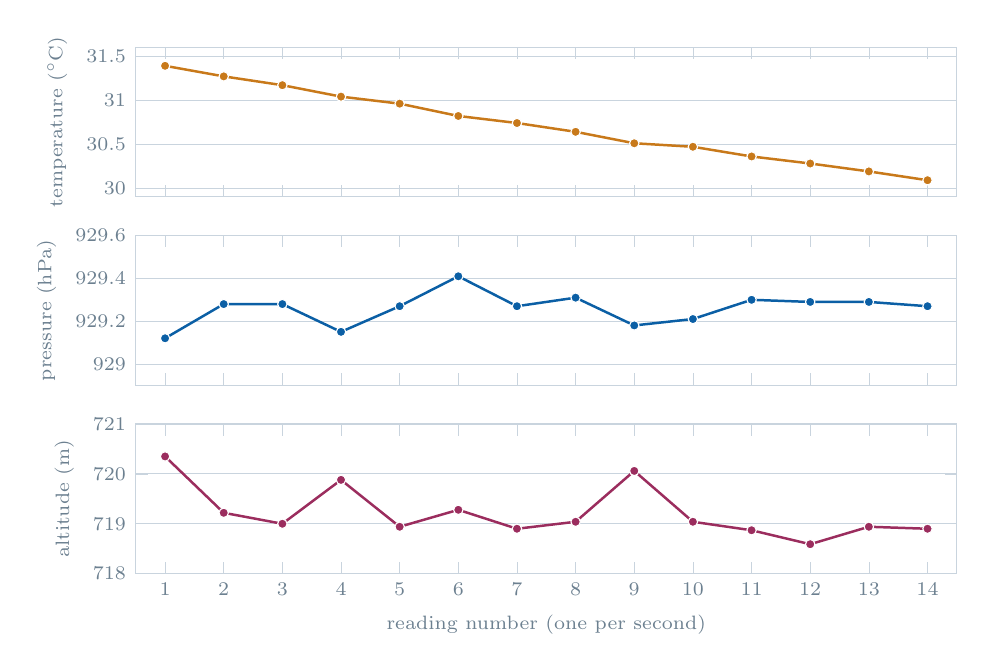
\begin{tikzpicture}
\begin{groupplot}[
  group style={group size=1 by 3, vertical sep=14pt, x descriptions at=edge bottom},
  width=0.86\textwidth, height=1.9cm, scale only axis,
  xmin=0.5, xmax=14.5, xtick={1,2,...,14},
  tick label style={font=\scriptsize, color=cmnt},
  axis line style={rule, line width=0.4pt}, tick style={rule},
  ymajorgrids, grid style={rule, line width=0.3pt},
  ylabel style={font=\scriptsize, color=cmnt},
  xlabel={reading number (one per second)}, xlabel style={font=\scriptsize, color=cmnt},
  clip=false]
\nextgroupplot[ymin=29.9, ymax=31.6, ytick={30.0,30.5,31.0,31.5}, ylabel={temperature ($^{\circ}$C)}]
\addplot[amber, line width=0.9pt, mark=*, mark size=1.7pt, mark options={fill=amber, draw=white, line width=0.4pt}]
  coordinates {(1,31.39) (2,31.27) (3,31.17) (4,31.04) (5,30.96) (6,30.82) (7,30.74)
               (8,30.64) (9,30.51) (10,30.47) (11,30.36) (12,30.28) (13,30.19) (14,30.09)};
\nextgroupplot[ymin=928.9, ymax=929.6, ytick={929.0,929.2,929.4,929.6}, ylabel={pressure (hPa)},
               yticklabel style={/pgf/number format/fixed, /pgf/number format/precision=1}]
\addplot[accent, line width=0.9pt, mark=*, mark size=1.7pt, mark options={fill=accent, draw=white, line width=0.4pt}]
  coordinates {(1,929.12) (2,929.28) (3,929.28) (4,929.15) (5,929.27) (6,929.41) (7,929.27)
               (8,929.31) (9,929.18) (10,929.21) (11,929.30) (12,929.29) (13,929.29) (14,929.27)};
\nextgroupplot[ymin=718, ymax=721, ytick={718,719,720,721}, ylabel={altitude (m)}]
\addplot[num, line width=0.9pt, mark=*, mark size=1.7pt, mark options={fill=num, draw=white, line width=0.4pt}]
  coordinates {(1,720.35) (2,719.22) (3,719.00) (4,719.88) (5,718.94) (6,719.28) (7,718.90)
               (8,719.04) (9,720.06) (10,719.04) (11,718.87) (12,718.59) (13,718.94) (14,718.90)};
\end{groupplot}
\end{tikzpicture}
\caption{The 14 readings of the Raspberry Pi run. The temperature falls steadily as the
module cools after being handled; the pressure is flat to within $\pm0.15\,\mathrm{hPa}$,
and the altitude, computed from it, jitters by about a metre around $719\,\mathrm{m}$.}
\label{fig:pi-trend}
\end{figure}

\begin{figure}[H]
\centering
\begin{minipage}[t]{0.575\textwidth}
\centering
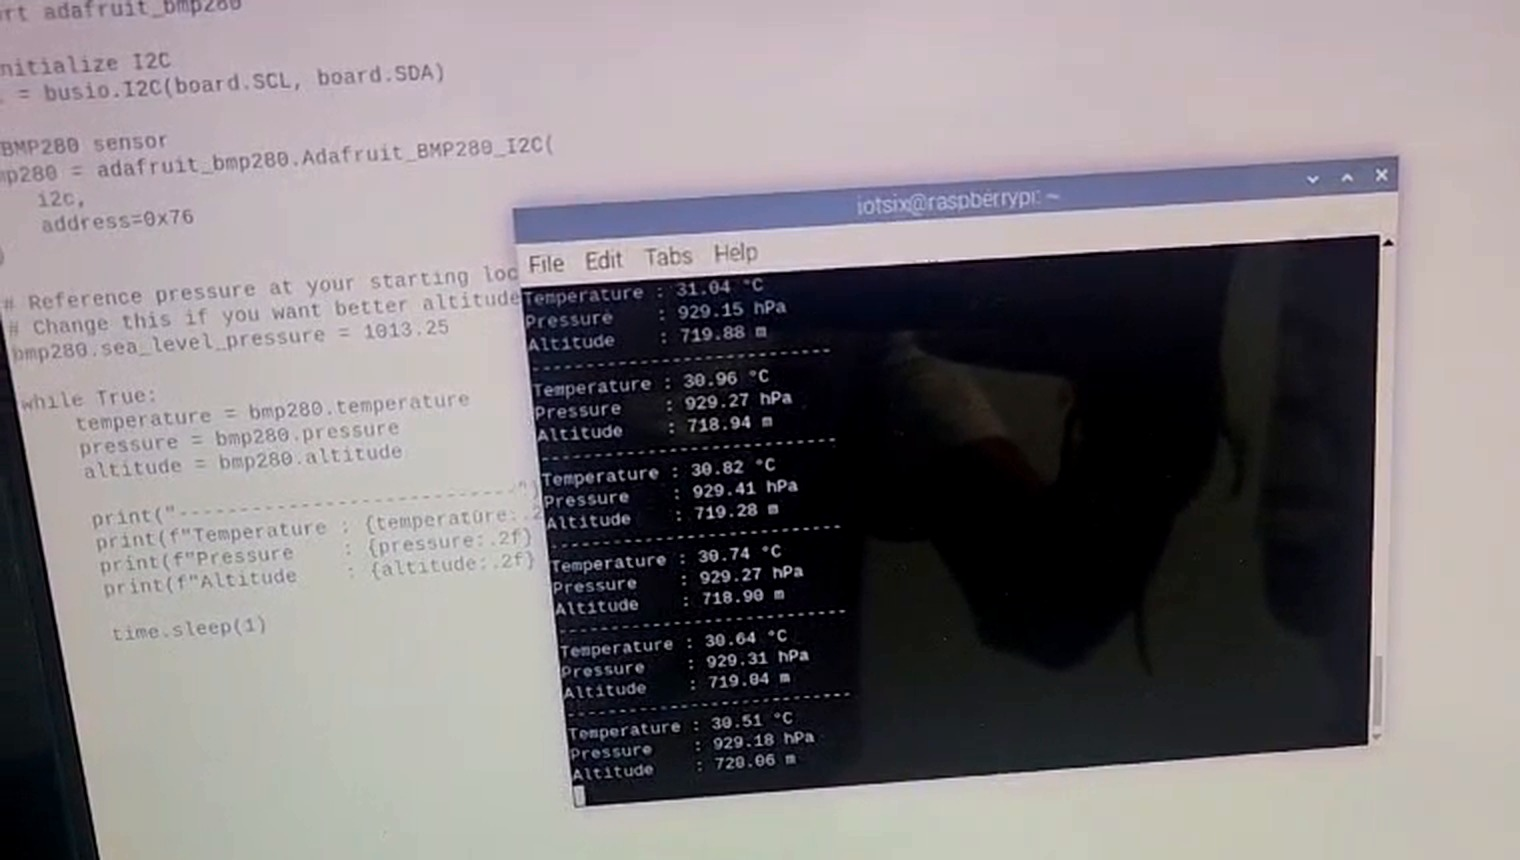
\includegraphics[width=\linewidth]{figures/rpi_editor_terminal.jpg}
\end{minipage}\hfill
\begin{minipage}[t]{0.405\textwidth}
\centering
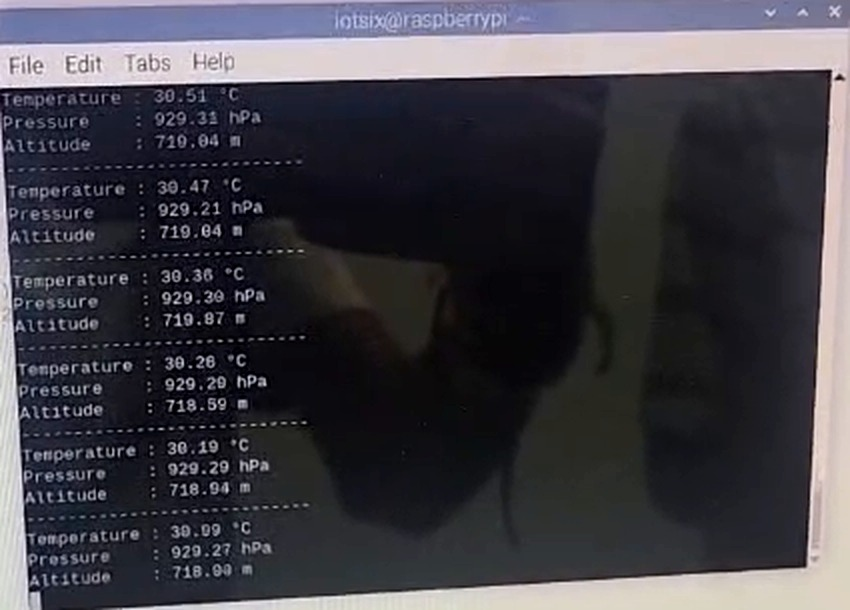
\includegraphics[width=\linewidth]{figures/rpi_terminal_2.jpg}
\end{minipage}
\caption{Part A on screen. \emph{Left:} \texttt{pressure.py} open in the editor behind
the terminal, which is printing the readings; \emph{right:} a later frame with the last
readings of the run. Each block is one second's temperature, pressure and altitude.}
\label{fig:pi-terminal}
\end{figure}

\subsection*{Observed outputs --- Part B, ESP32 dashboard}

\vspace{2pt}
\noindent
\begin{minipage}[t]{0.53\textwidth}
\vspace{0pt}
\begin{tabularx}{\linewidth}{@{}l c c >{\centering\arraybackslash}X@{}}
\toprule
\rowcolor{soft}
\textbf{Clip time} & \textbf{Temp.\ ($^{\circ}$C)} & \textbf{Pressure (hPa)} & \textbf{Altitude (m)} \\
\midrule
0\,s  & 24.53 & 940.19 & 626.83 \\
1\,s  & 24.53 & 940.18 & 626.97 \\
2\,s  & 24.54 & 940.22 & 626.57 \\
6\,s  & 24.54 & 940.20 & 626.76 \\
8\,s  & 24.54 & 940.15 & 627.16 \\
10\,s & 24.56 & 940.14 & 627.31 \\
12\,s & 24.57 & 940.15 & 627.19 \\
16\,s & 24.58 & 940.19 & 626.82 \\
\midrule
clip 2, 7\,s & 24.60 & 940.10 & 627.62 \\
clip 2, 8\,s & 24.60 & 940.13 & 627.34 \\
\bottomrule
\end{tabularx}
\end{minipage}\hfill
\begin{minipage}[t]{0.43\textwidth}
\vspace{0pt}
\begin{titledbox}[unbreakable]{Checking the altitude}
\raggedright
For the first dashboard value, $p = 940.19\,\mathrm{hPa}$:
\[
  h = 44330\Bigl[1-\Bigl(\tfrac{940.19}{1013.25}\Bigr)^{1/5.255}\Bigr] = 626.8\,\mathrm{m},
\]
exactly the $626.83\,\mathrm{m}$ shown. The same check on the Pi's $929.27\,\mathrm{hPa}$
gives $724\,\mathrm{m}$, within a few metres of the printed $719\,\mathrm{m}$ --- the Pi
library takes a fresh pressure sample for the altitude, so the two lines are not from
the identical measurement.
\end{titledbox}
\end{minipage}

\vspace{6pt}
\noindent Values read from the dashboard in the two recorded clips. The temperature is
six degrees lower than in Part A because this run took place in the air-conditioned
lab a week earlier with the module untouched on the desk, and the pressure is
$11\,\mathrm{hPa}$ higher --- a different day's weather --- which the formula turns into
an ``altitude'' $92\,\mathrm{m}$ lower for the same room.

\begin{figure}[H]
\centering
\begin{minipage}[t]{0.29\textwidth}
\centering
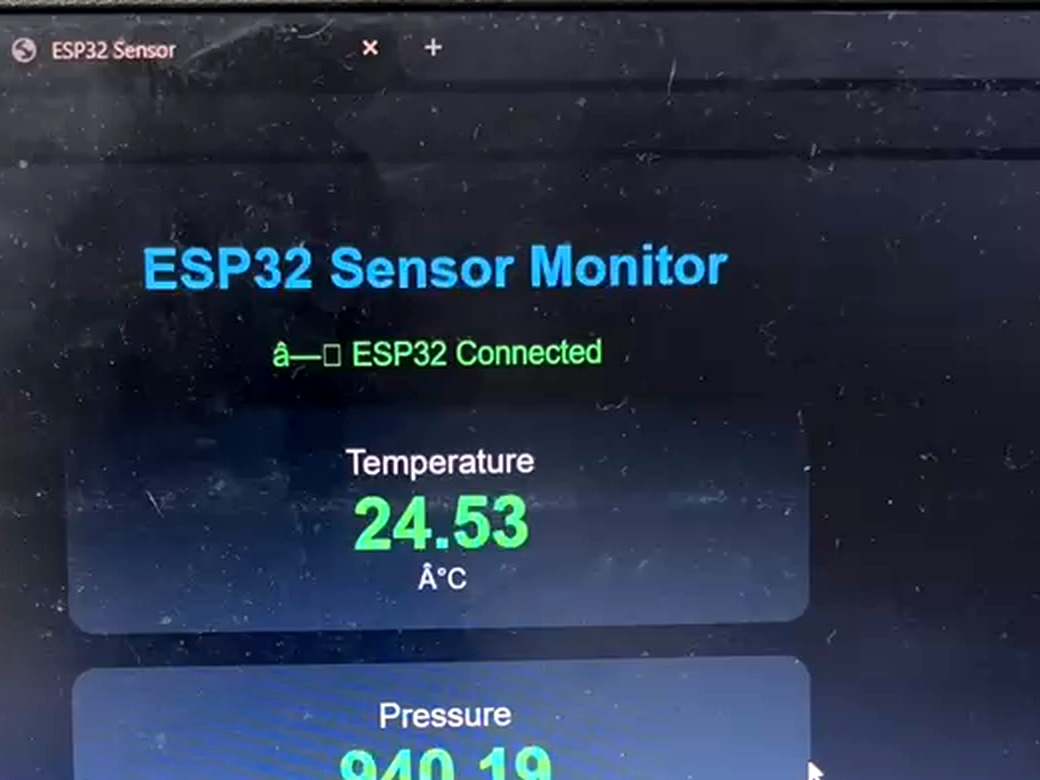
\includegraphics[width=\linewidth]{figures/esp32_dashboard_a.jpg}\\[2pt]
{\scriptsize\color{cmnt} first clip, $t=0$}
\end{minipage}\hfill
\begin{minipage}[t]{0.29\textwidth}
\centering
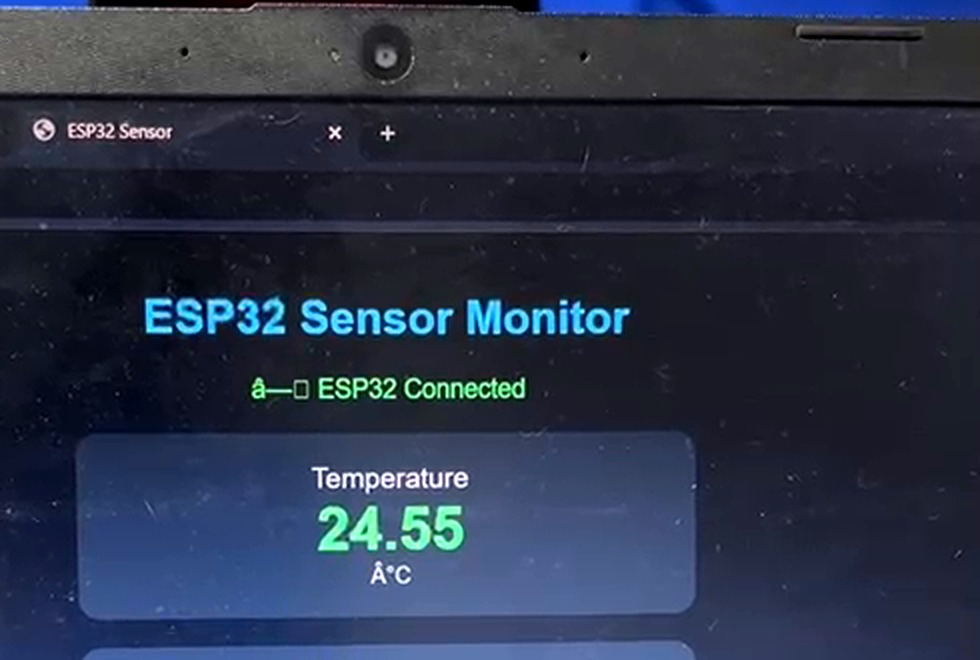
\includegraphics[width=\linewidth]{figures/esp32_dashboard_b.jpg}\\[2pt]
{\scriptsize\color{cmnt} first clip, $t=9\,$s}
\end{minipage}\hfill
\begin{minipage}[t]{0.39\textwidth}
\centering
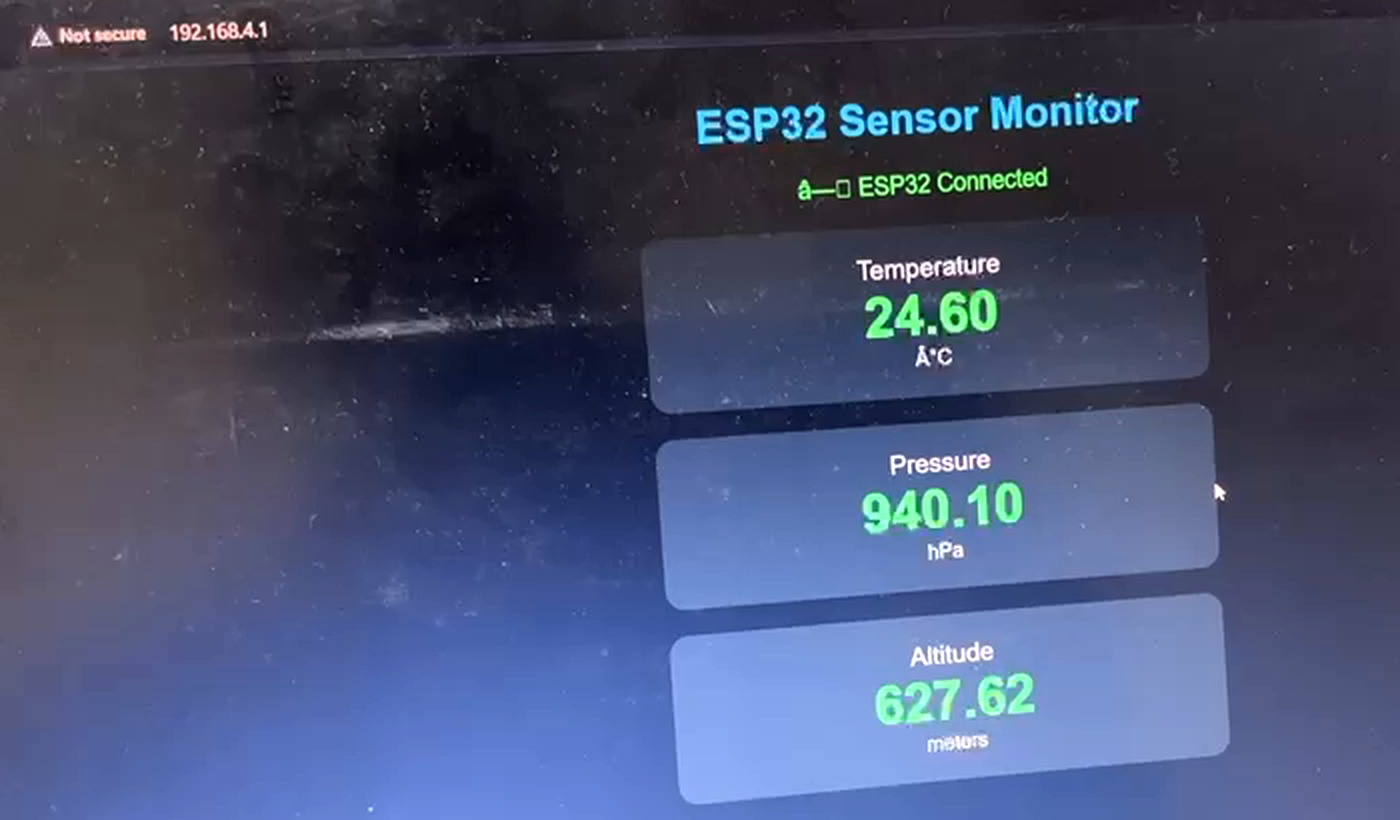
\includegraphics[width=\linewidth]{figures/esp32_dashboard_c.jpg}\\[2pt]
{\scriptsize\color{cmnt} second clip --- address bar shows \texttt{192.168.4.1}}
\end{minipage}
\caption{Part B. The dashboard served by the ESP32, viewed in the laptop's browser at
the access point's address \texttt{192.168.4.1}: the ``ESP32 Connected'' indicator and
three cards whose values change every second. (The stray \texttt{\^{A}} before the
degree sign in the recording is a character-encoding slip in the page as run that day;
see the Discussion.)}
\label{fig:dashboard}
\end{figure}

\subsection*{The setups}

\begin{figure}[H]
\centering
\begin{minipage}[t]{0.30\textwidth}
\vspace{0pt}
\centering
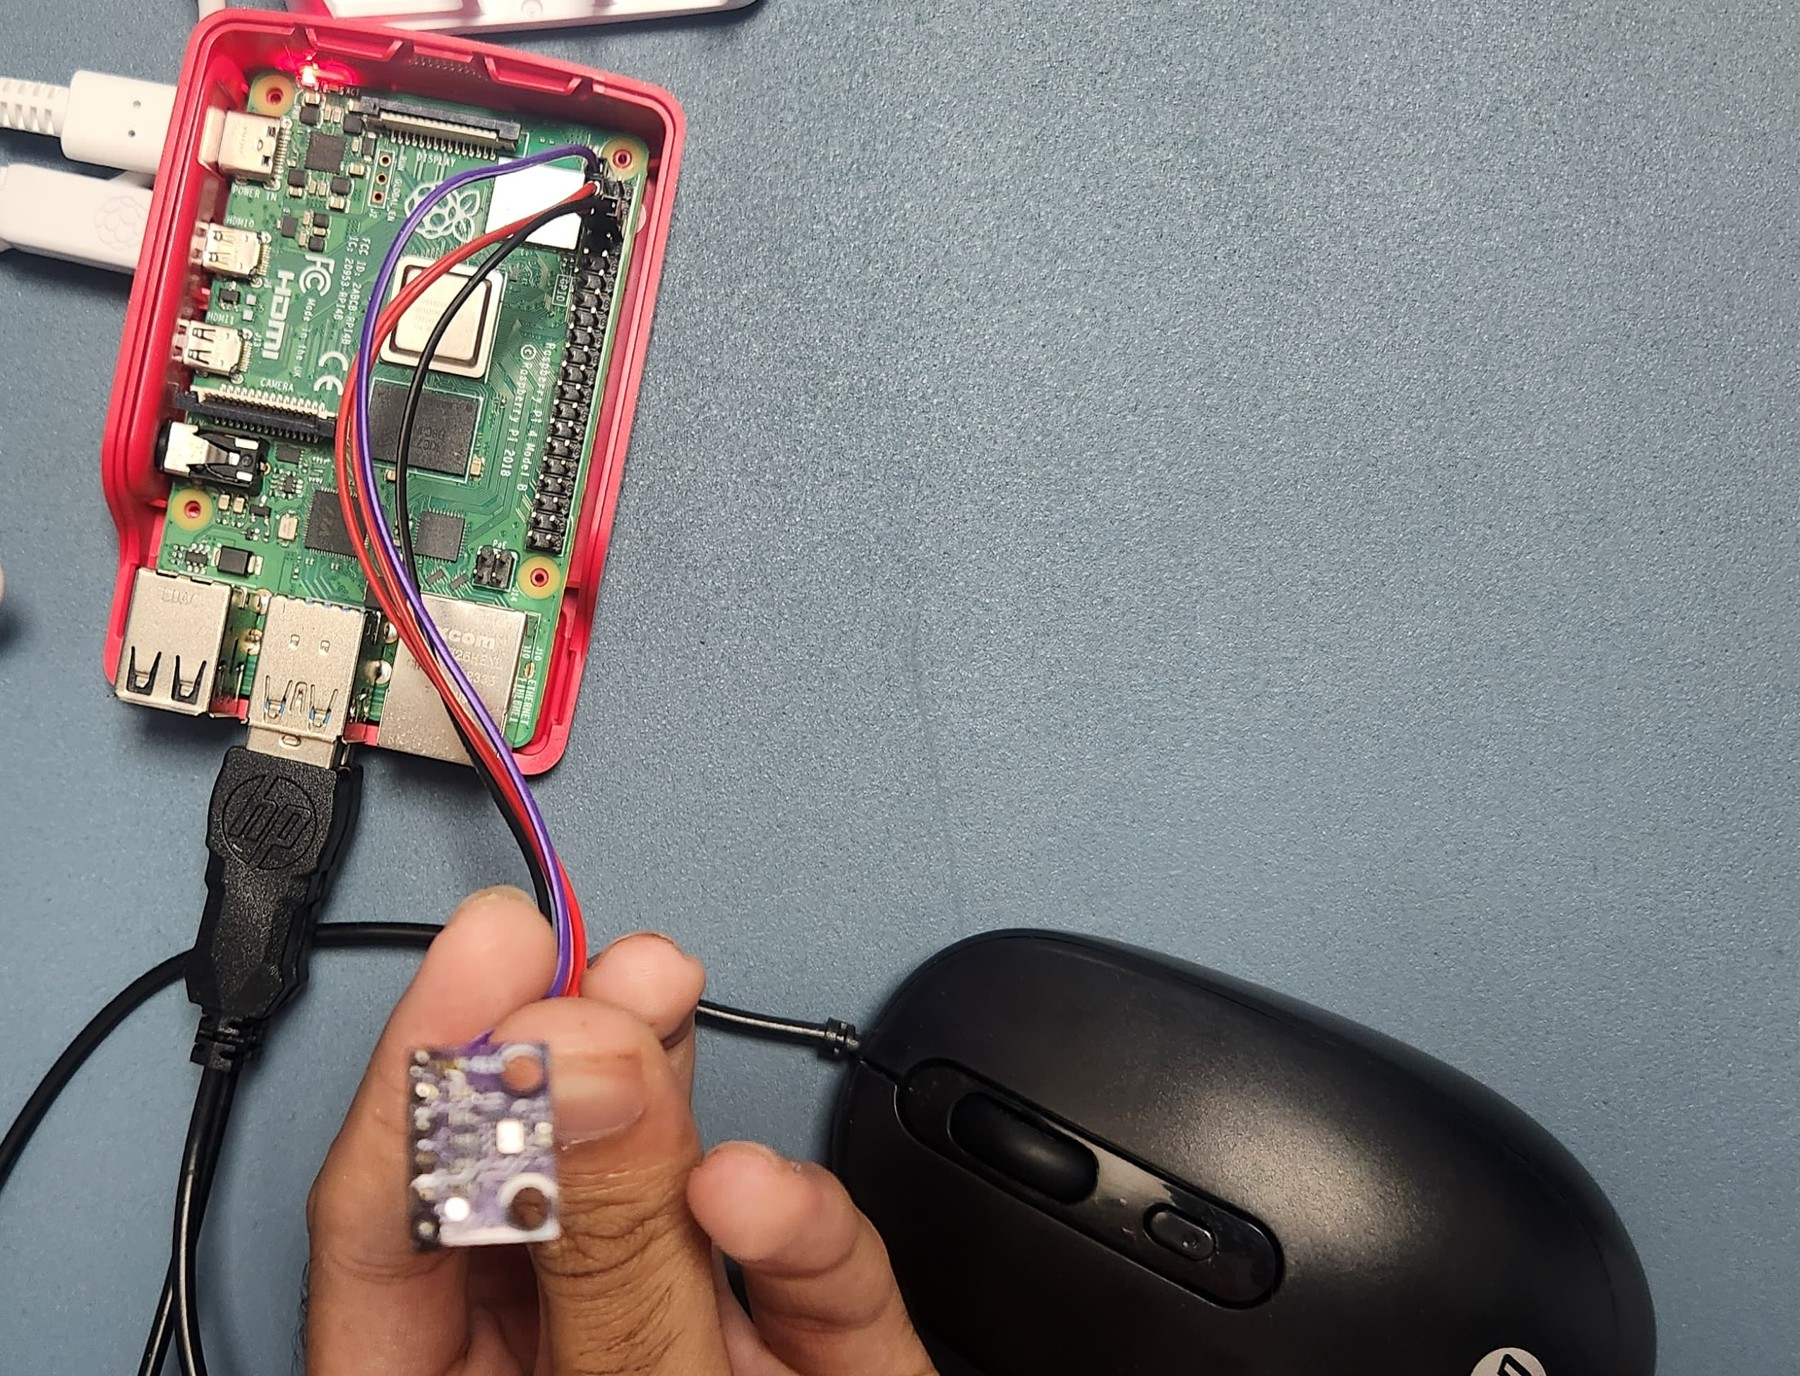
\includegraphics[width=\linewidth]{figures/rpi_bmp280_setup.jpg}
\end{minipage}\hfill
\begin{minipage}[t]{0.30\textwidth}
\vspace{0pt}
\centering
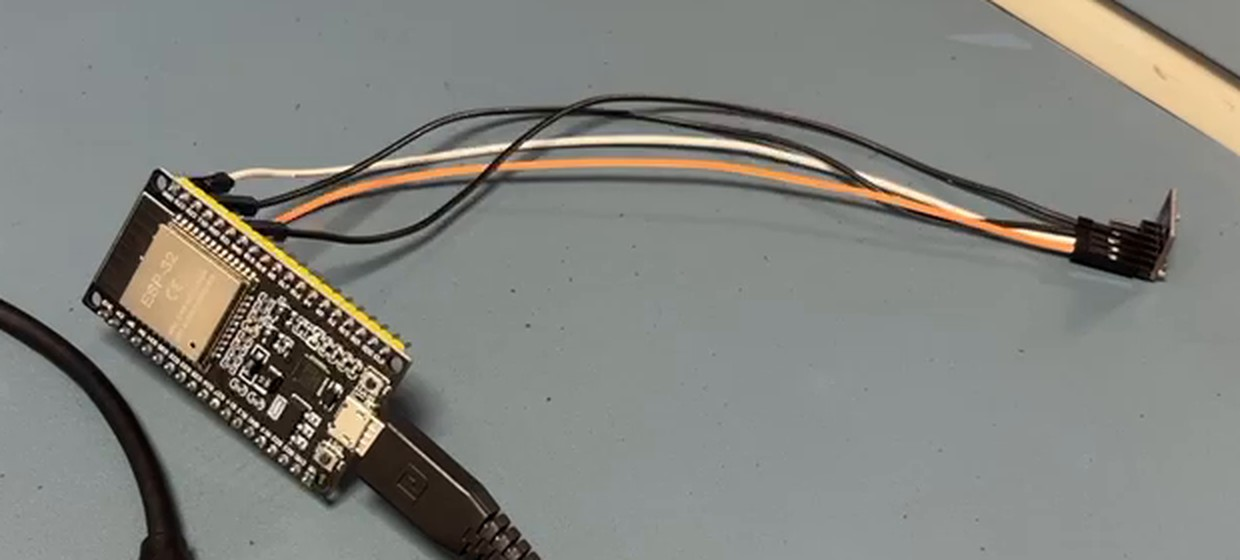
\includegraphics[width=\linewidth]{figures/esp32_bmp280_wiring.jpg}
\end{minipage}\hfill
\begin{minipage}[t]{0.175\textwidth}
\vspace{0pt}
\centering
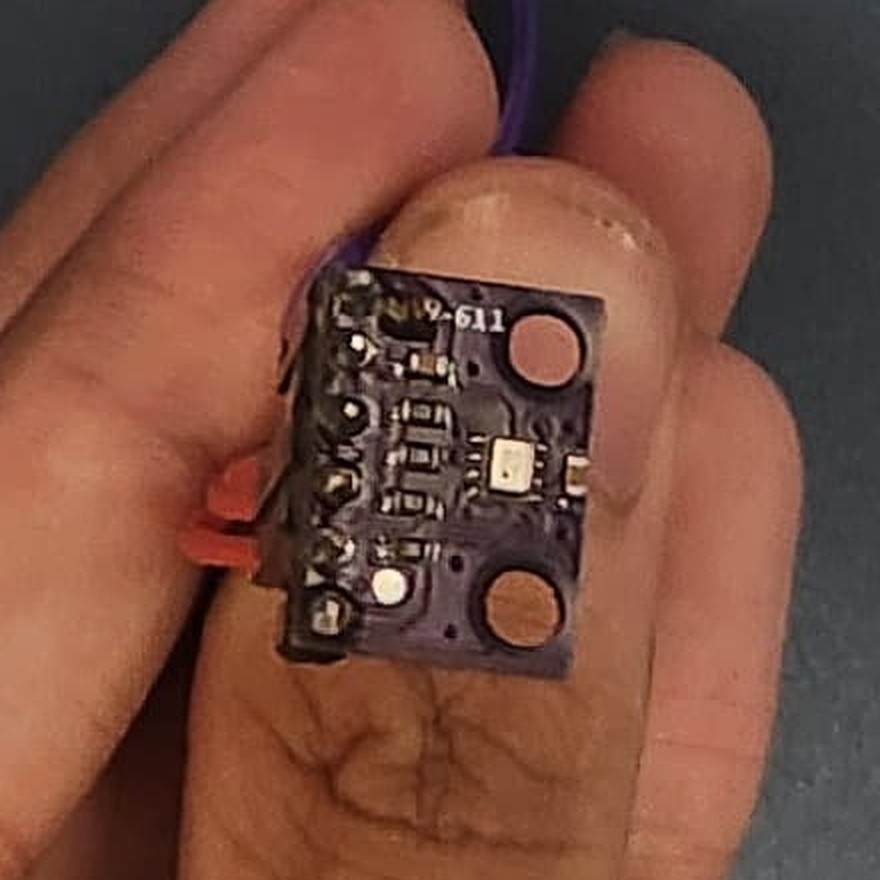
\includegraphics[width=\linewidth]{figures/bmp280_module.jpg}
\end{minipage}
\caption{\emph{Left:} Part A --- the Raspberry Pi 4 with the BMP280 module on four
jumper wires. \emph{Centre:} Part B --- the ESP32 DevKit with the same module.
\emph{Right:} the six-pin breakout with the BMP280 (the small metal package).}
\label{fig:setups}
\end{figure}

\subsection*{Video demonstration and code}

\begin{titledbox}[before skip=6pt]{Google Drive link}
\noindent The demonstration videos, this report and the complete source code are
available in the following shared folder:

\vspace{4pt}
\noindent\drivefolder

\vspace{4pt}
{\small\color{cmnt} Access has been set to \emph{anyone with the link can view}.}
\end{titledbox}

\subsection*{Discussion}
\label{sec:discussion}
\begin{itemize}
  \item \textbf{What the altitude really is.} The same room gave $719\,\mathrm{m}$ on one
        day and $627\,\mathrm{m}$ on another, and Indore actually lies at roughly
        $550\,\mathrm{m}$. None of these is a sensor fault: the formula assumes a
        sea-level pressure of $1013.25\,\mathrm{hPa}$, and on both days --- in the monsoon
        season --- it was lower, by different amounts. A barometric altimeter must
        therefore be given the \emph{actual} sea-level pressure (the ``QNH'' from a weather
        station) through \texttt{sea\_level\_pressure}, after which it reads true altitude;
        or it is used for \emph{relative} height, where the reference cancels and the
        $\pm0.12\,\mathrm{hPa}$ resolution gives about one metre.
  \item \textbf{Noise and averaging.} Successive pressure readings scatter by
        $\pm0.15\,\mathrm{hPa}$, which is $\pm1.3\,\mathrm{m}$ of altitude --- visible as the
        jitter in Figure~\ref{fig:pi-trend} and in the dashboard's last digits. The
        BMP280's oversampling and on-chip IIR filter, or a software average, smooth it.
  \item \textbf{Temperature is the chip's, not the room's.} The BMP280 measures its own
        die temperature, mainly to compensate the pressure. It reads high when the module
        is warm: $31\,^{\circ}\mathrm{C}$ and falling in Part A right after the module had
        been held, $24.5\,^{\circ}\mathrm{C}$ and steady in Part B on the desk in the
        air-conditioned lab.
  \item \textbf{Two ways to deliver the data.} The Pi prints to its own terminal, which
        needs a screen; the ESP32 has no screen but has Wi-Fi, so it serves the data as
        a web page. As an access point it works anywhere, without a router --- the laptop
        joins the ESP32's network and opens \texttt{192.168.4.1}. Polling a small JSON
        endpoint once a second is the same pattern an IoT node uses to report to a server.
  \item \textbf{The stray character.} The recorded dashboard shows ``\^{A}°C'': the page
        sent a raw degree sign without declaring its encoding, so the browser read its two
        UTF-8 bytes as two Latin-1 characters; Listing~\ref{lst:esp} declares the charset.
  \item \textbf{I$^2$C versus one-wire.} Unlike the DHT11, the BMP280 never returned a
        bad frame: I$^2$C is clocked by the master, so the operating system's timing
        jitter cannot corrupt the data, and the hardware peripheral does the bit-level work.
\end{itemize}

%------------------------------------------------------------------ CONCLUSION
\Needspace{10\baselineskip}
\section{Conclusion}

The BMP280 was read successfully from both a Raspberry Pi and an ESP32 over the
I$^2$C bus, giving calibrated pressure and temperature and a derived altitude. The
Raspberry Pi printed a clean, steady stream of readings --- $929.3\,\mathrm{hPa}$, about
$719\,\mathrm{m}$ pressure altitude, temperature settling from $31.4$ to
$30.1\,^{\circ}\mathrm{C}$ --- and the ESP32 delivered the same three quantities as a
live web dashboard on its own Wi-Fi network, at $940.2\,\mathrm{hPa}$ and
$627\,\mathrm{m}$ on a different day; every altitude value reproduced the barometric
formula applied to its pressure.

The experiment made two points concrete: a barometric altitude is a pressure
measurement in disguise, and depends on the sea-level reference as much as on height;
and a hardware bus such as I$^2$C is a far more robust way to attach a sensor than the
timing-critical one-wire link of the previous experiment. The ESP32 part also took the
first step from reading a sensor to \emph{publishing} its data over a network --- the
essence of an IoT node.

\end{document}
